\part*{آزمایش اجرای نرم افزار تحت وب }
\chapter*{معرفی}
\section{نصب و اجرای وردپرس 
    \lr{WordPress}
      برای آزمودن کارساز}
 وردرپرس «\lr{Wordpress}» نرم‌افزاری تحت وب و متن‌باز است که برای مدیریت محتوا در اینترنت بسیار کاربرد دارد، حال اگر می‌خواهید قالب طراحی کنید یا این‌که در توسعهٔ وردپرس فارسی یا خود وردپرس مشارکت داشته باشید و .. می‌توانید آن را در این سندباکس نصب کنید، تنها کافی است آن را از پایگاه اینترنتی وردپرس \lr{WordPress} بارگیری کنید و سپس در شاخهٔ سندباکس «\path{/media/sf_sandbox}» رونویسی و درج کنید، بعد از آن یک نام کاربری به همراه پایگاه داده با نام «\lr{wordpress}»  یا هرچه که دوست دارید، بسازید و در هنگامی که مراحل نصب وردپرس نمایش داده می‌شود وارد کنید. بعد از آن اگر مراحل قبلی این آموزش از قسمت اول را دنبال کرده باشید به راحتی وردپرس اجرا می‌شود، مثالی از اجرای وردپرس در سندباکس در بالا قابل مشاهده است.
\begin{figure}
    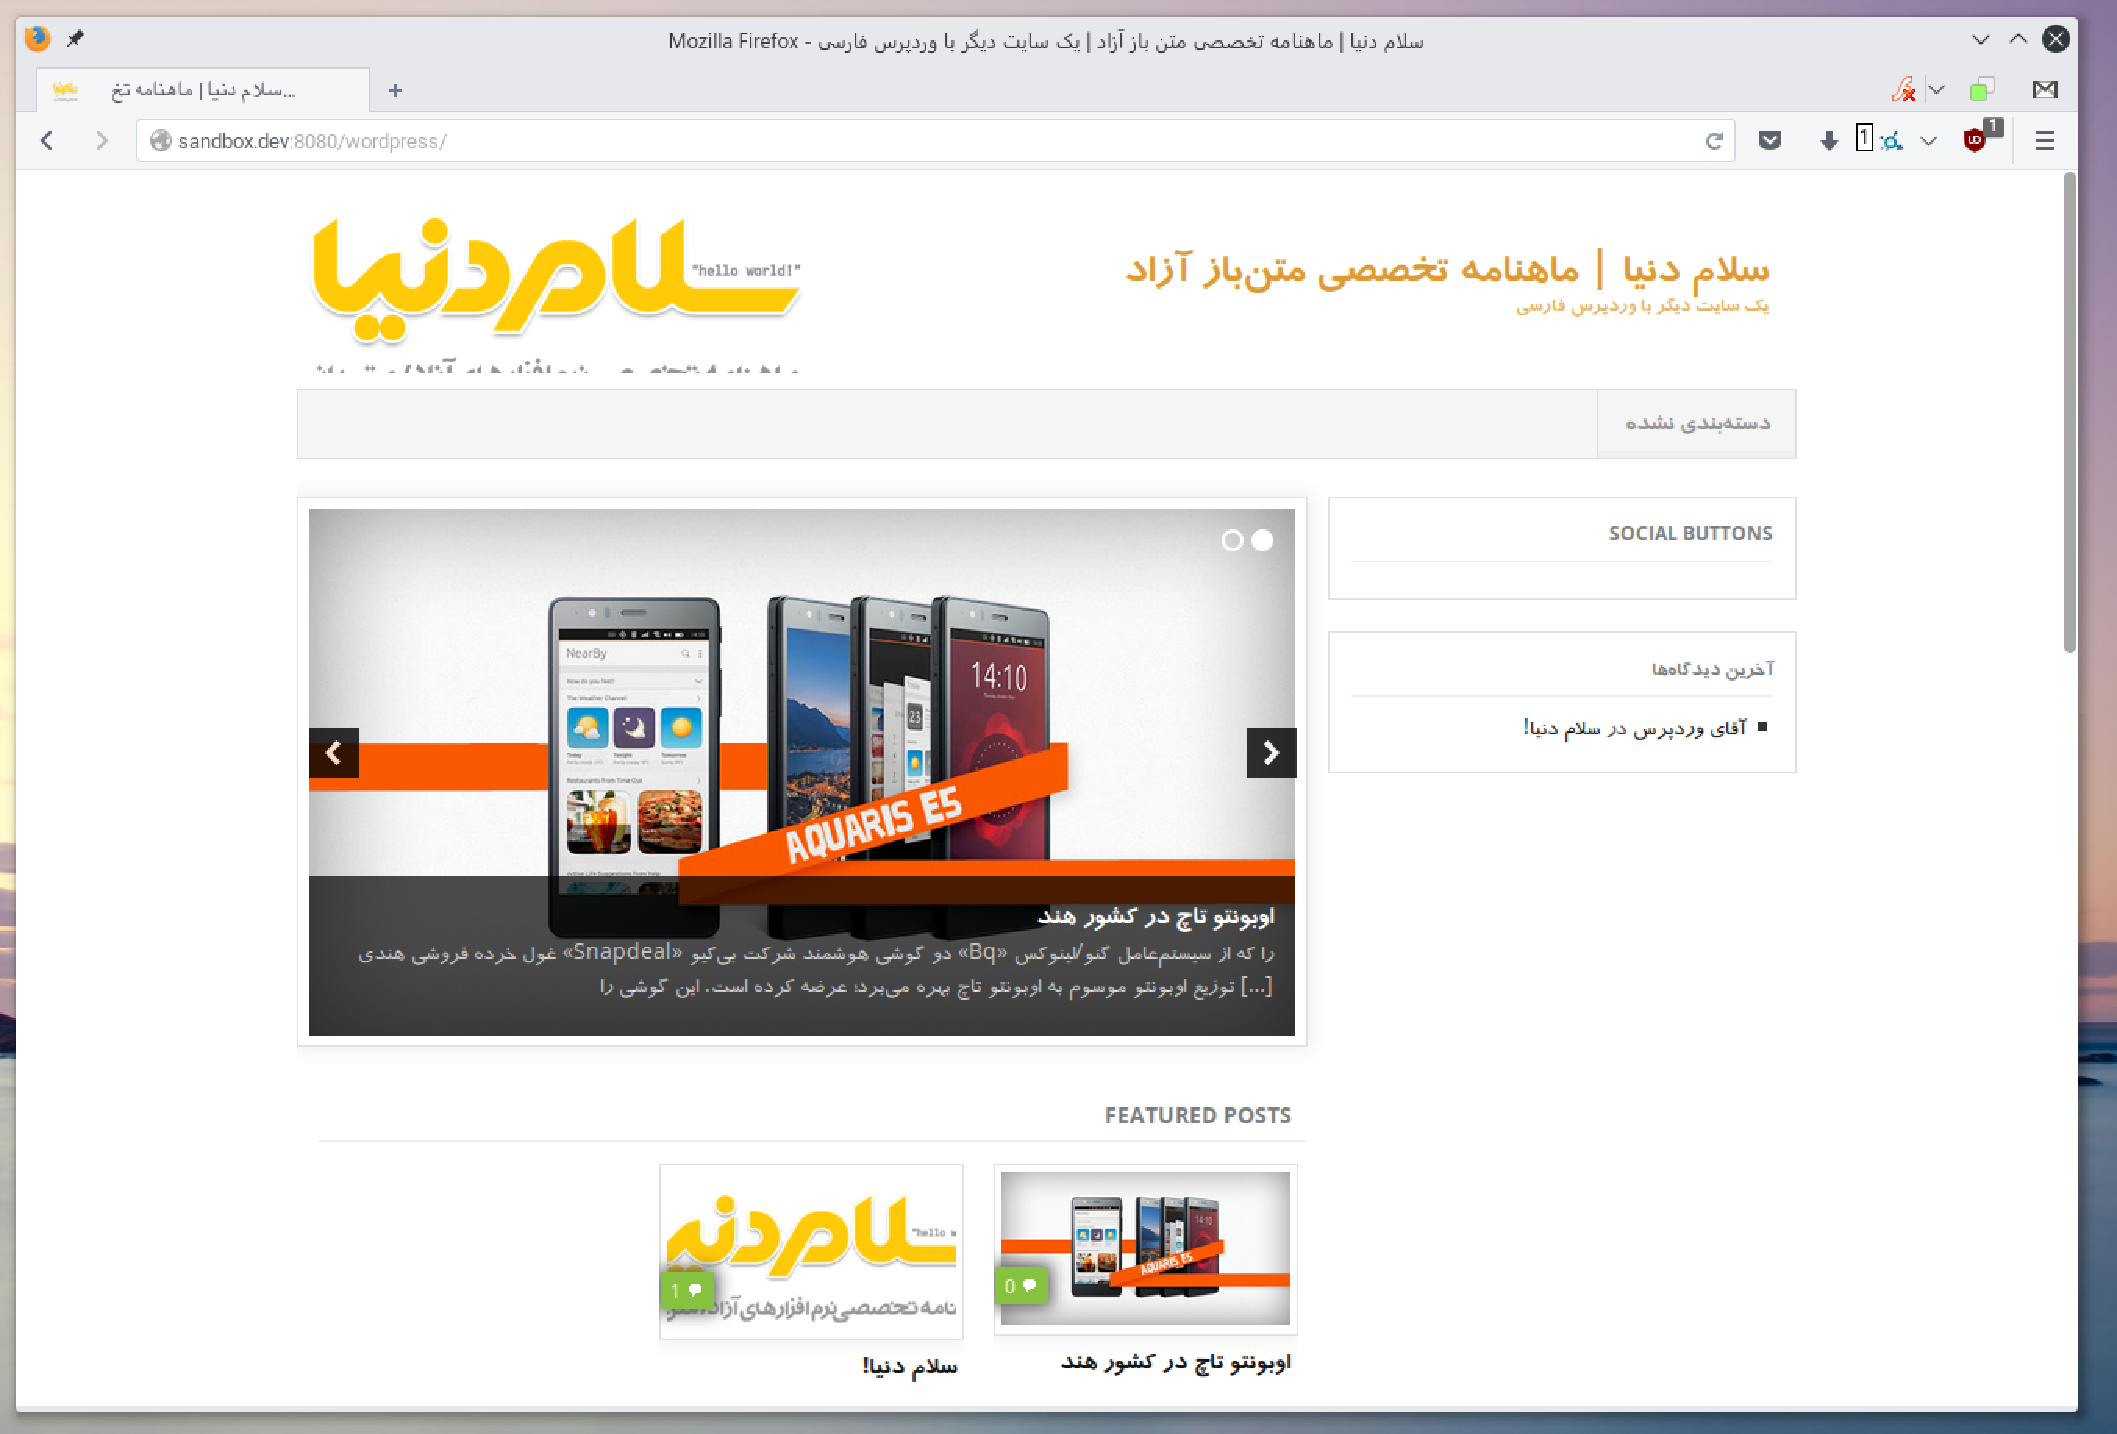
\includegraphics[width=.9\textwidth ,height=.50\textwidth]{Pic/WP-SANDBOX}
    \caption{ نمایی از وردپرس که در سندباکس نصب شده است
        \lr{}   
    }
    \label{WP-SANDBOX}
\end{figure}

\section{نصب مدیر محتوای آزاد دروپال}

\begin{figure}
    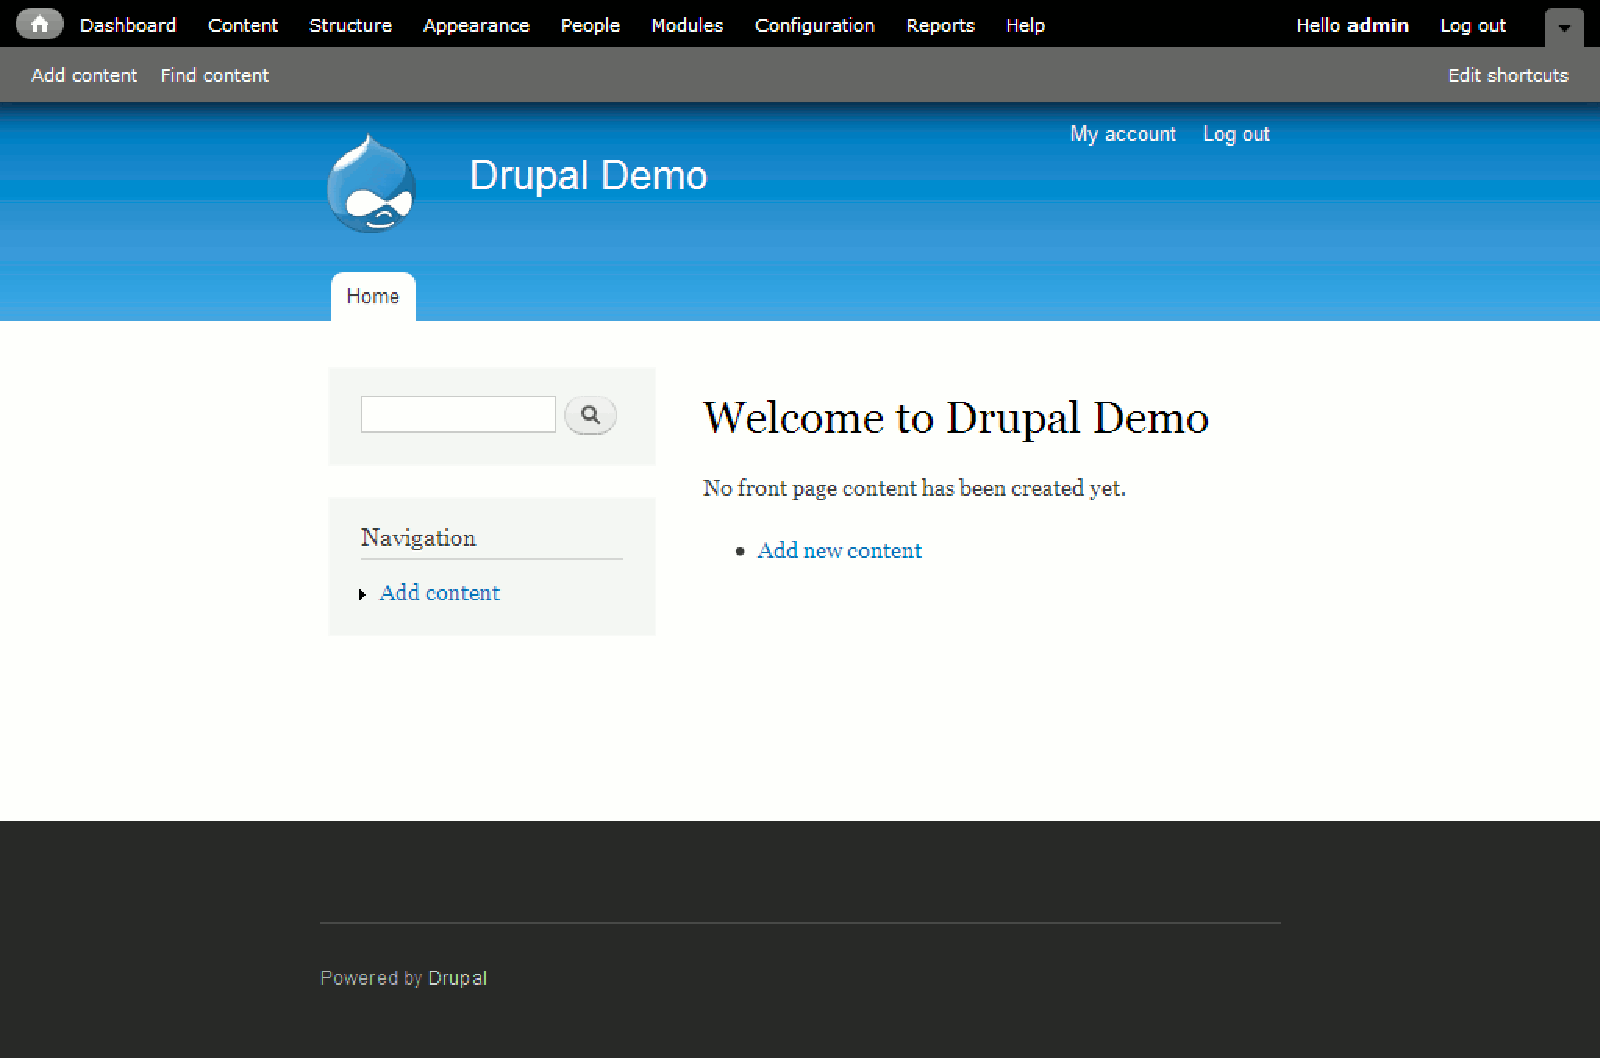
\includegraphics[width=.9\textwidth ,height=.50\textwidth]{Pic/DRUPAL2}
    \caption{ نمایی از دروپال که در حال اجرا است.
        \lr{}   
    }
    \label{DRUPAL-SANDBOX2}
\end{figure}
دروپال سامانه مدیریت محتوایی آزاد و متن‌باز به زبان پی‌اچ‌پی است که برای توسعه برنامه‌های کاربردی مبتنی بر وب و ایجاد بلاگ است که تحت مجوز جی‌پی‌ال منتشر شده‌است. از این برنامه برای مدیریت محتوای بیش از ۱ درصد از صفحات وب استفاده شده است. از این سیستم مدیریت محتوا از وبلاگ‌های شخصی تا شرکت‌های تجاری، سیاسی و حتی دولت‌ها نیز استفاده شده است. وبگاه کاخ سفید و  انگلستان 
[\url{http://data.gov.uk} \url{http://data.gov.uk}]
 نیز از دروپال استفاده می‌کنند.

\begin{figure}
    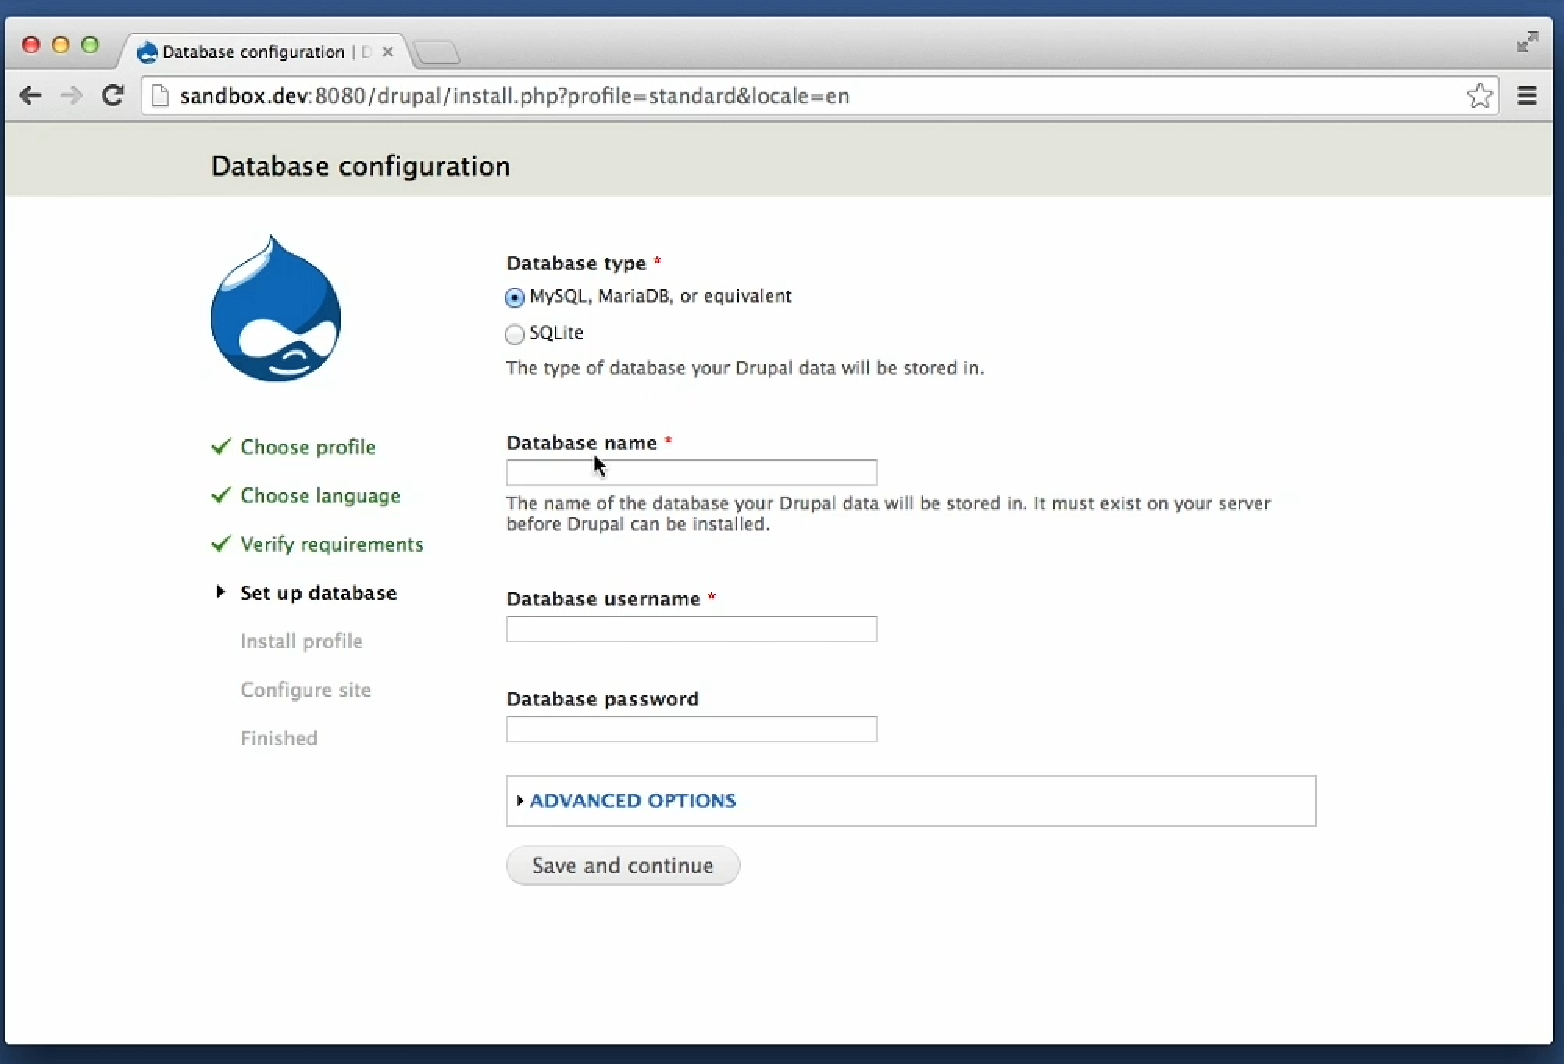
\includegraphics[width=.9\textwidth ,height=.50\textwidth]{Pic/DRUPAL}
    \caption{ نمایی از دروپال که در سندباکس در حال نصب است.
        \lr{}   
    }
    \label{DRUPAL-SANDBOX}
\end{figure}

دروپال را می‌توان در سیستم‌عامل‌های مختلف نصب نمود. پیش نیازهای نصب این برنامه یک کارگزار وب مانند آپاچی و یک پایگاه داده مانند 
\lr{MySQL}
 می‌باشند. همچنین می‌بایست که پی‌اچ‌پی ۴.۴.۰ یا نسخه‌ی جدید تر نصب باشد. البته در نسخه‌ی ۷ دروپال نسخه‌ی پی‌اچ‌پی ۵.۲ یا بالاتر مورد نیاز است.
نسخه استاندارد دروپال که هسته دروپال شناخته می‌شود، ویژگی‌های پایه معمول یک سیستم مدیریت محتوا را داراست. این‌ها شامل ثبت نام کاربری و تعمیر، مدیریت منو، خوراک آراس‌اس، رده‌بندی، شخصی‌سازی ساختار برگه و مدیریت سیستم می‌شود. هسته دروپال می‌تواند برای یک وبسایت ساده، وبلاگ تکی و گروهی، فروم اینترنتی یا انجمنی اینترنتی که محتوای آن توسط کاربران ایجاد شود به کار رود. 
\begin{flushleft}
    (ویکی‌پدیا دانشنامهٔ آزاد)
\end{flushleft}

\part*{سخن پایانی}
\chapter*{نتیجه‌گیری}
این مجموعهٔ آموزشی در این قسمت به پایان رسید، بعد از شش قسمت آموزشی به راحتی می‌توانید نرم‌افزارها یا صفحات اینترنتی خود را درون سندباکس توسعه داده و اجرا کنید. اوبونتو سرور به عنوان یک توزیع محبوب در رایانه‌های کارساز وب شناخته می‌شود که کارکردی بسیار آسان درد، این آموزش برای شما دو منفعت خواهد داشت، نخست آن‌که به راحتی می‌توانید در آن کدها و صفحات اینترنتی نوشته‌شدهٔ خود را مشاهده و آزمایش کنید و سپس به راحتی با هزینه‌ای اندک از ایراد و اشکالات کار خود با خبر شوید. سپس ویژگی بعدی آن که این آموزش را از دیگر آموزه‌های اجرا و نصب 
\lr{LAMP}
 برتری می‌دهد، آموزش کامل نصب، اجرا و تنظیم یک کارساز وب اوبونتو برای توسعهٔ نرم‌افزار به زبان پی‌اچ‌پی است که باعث می‌شود، در آینده اگر خواستید کارساز وب واقعی را راه‌اندازی کنید، با مشکلات کمتری مواجه باشید.

یادگیری و استفاده از نرم‌افزارهای آزاد ممکن است در ابتدا کمی مشکل باشند، با این حال این زمانی که صرف تنظیم نرم‌افزاری آزاد می‌کنید را می‌توانید بهای آزادی و امنیّت بدانید. ممکن است موارد ذکر شده در این آموزش را در برخی ابزارهای غیر آزاد/متن‌باز به راحتی در اختیار داشته باشید، اما اگر خودتان با استفاده از نرم‌افزار آزاد چنین کارهایی را انجام دهید، نسخت دانش خود را افزایش داده‌اید و سپس امنیّت و حریم خصوص خود را حفظ کرده‌اید. بنابراین فقط به دلیل این‌که مورد بالا ممکن است کمی طولانی باشند از امتحان کردن آن خودداری نکنید. این موضوع برای دیگر نرم‌افزارهای آزاد در مقابل نرم‌افزارهای انحصاری دیگر نیز صادق است. با این حال از تمامی دوستان تقاضا دارم، انتقادات و پیشنهادات خود را در این مورد با توییتر بنده با رایا‌نامه بنده در میان بگزارید.

در پایان از پایگاه اینترنتی سلام دنیا، محمد دماوندی و بهنام توکلی عزیز به دلیل ایجاد امکانات و بستر مناسب برای عرضهٔ این آموزش کمال تشکر را داشته و از شما خوانندگان عزیز به دلیل مطالعهٔ این آموزش  و نظرات دلگرم‌کنندهٔ خود در توییتر و جی‌میل تشکر می‌کنم.

\chapter*{حمایت مالی :}
کدهایی که برای ایجاد پی‌دی‌اف در زی‌لاتک نوشته شده‌اند را نیز به صورت کامل در پایگاه اینترنتی گیت‌هاب بارگزاری می‌کنم تا در صورت نیاز بتوانید آن را برای نیاز خودتان تغییر دهید، همچنین در آینده نسخهٔ وبی از آن نیز ممکن است عرضه شود. اگر از سیستم‌عامل گنو/لینوکس استفاده می‌کنید، نرم‌افزار «TeXStudio» نرم‌افزار خوبی برای نوشتن و گرفتن خروجی پی‌دی‌اف از کدهای لاتک و زی‌لاتک به شمار می‌آید،خودم شخصاً نتوانستم از طریق نرم‌افزارهای دیگر در نو/لینوکس این کار را انجام دهم. توزیع من برای نوشتن لاتک و زی‌لاتک، توزیع آرچ لینوکس است و از نرم‌افزارهای پیش‌فرض موجود در داخل مخازن آرچ استفاده کرده‌ام.

همان‌طور که ذکر شد تمامی پرونده‌هایی که برای گرفتن خروجی PDF در زیلاتک نیاز باشد را در گیت‌هاب قرار خواهم داد، با این حال نسخهٔ PDF به صورت دیگر با شرایطی که ذکر خواهد شد، در اینترنت قرار می‌گیرد و نسخه‌ای چاپی از کتاب با دو کیفیت متفاوت نیز به فروش خواهد رسید که برای کاربرانی که می‌خواهند نسخهٔ چاپی کتاب را به‌همراه داشته باشند و با خرید خود کمک مالی کوچکی نیز به نویسنده داشته باشند، مناسب خواهد بود. با این وجود  دیگر کاربران نیز می‌توانند از طریق حسابی که بعداً در گیت‌هاب قرار خواهد گرفت به پروژه کمک کنند تا در آینده اگر کمک مالی مناسبی از جانب کاربران دریافت کردم، نسخهٔ ویدئویی آموزش را نیز ارائه دهم. به این دلیل که خوانندگان کاربران در توییتر و جی‌میل در خواست داشتند تا این آموزش به صورت ویدئویی ارائه شود تا بهتر بتوانند با آن ارتباط برقرار کنند. هر چند ارائه این ویدئوها با کیفیت مناسب نیازمند امکانات صوتی خوب و وقت بیشتر است، با این حال در صورت دریافت کمک‌های مالی در حد کفایت، این آموزش نیز در یوتیوب قرار خواهد گرفت.
